Электрический ток представляет собой направленный перенос зарядов. Микрочастицы,
осуществляющие этот перенос, называют \term{носителями тока}. В~простейшем
случае носителями тока являются заряженные частицы,
движущиеся в свободном от вещества пространстве (ток в вакуумном диоде,
ионный пучок в масс-спектрометре, и т.\,д.).
Как правило, это электроны~--- элементарные частицы с известными значениями заряда
$q_e=-e\approx-1,6\cdot 10^{-19}\;Кл$
и массы
$m_e\approx 9,1\cdot 10^{-31}\;кг$.

Понятие \term{носители тока в веществе} уже не является таким наглядным.
Хотя в металлах и полупроводниках перенос заряда происходит
вследствие перемещения всё тех же электронов, их движение уже не является
движением свободных частиц, как в вакууме. Электроны движутся в сильном
периодическом поле, образованном ионами кристаллической решётки, и
взаимодействуют между собой, причём это движение и это взаимодействие
подчиняются законам квантовой механики. По этим законам получается, что такое
движение можно по-прежнему интерпретировать как движение свободных заряженных
частиц, но масса этих частиц, называемая \term{эффективной массой},
\important{не совпадает с массой свободного электрона},
$m_{e}^{эфф}\ne m_e$.
Более того, полупроводники и некоторые металлы ведут себя так,
будто вместо электронов ток в них переносят некоторые положительные частицы~---
так называемые \term{дырки}. Дырки подобны элементарным
частицам позитронам~--- в электрических и магнитных полях они движутся
как положительно заряженные частицы с зарядом $q_p=+e$,
но с некоторой эффективной массой $m_p^{эфф}\ne m_e$.

Таким образом, в физике металлов и полупроводников в качестве носителей тока
рассматривают \term{квазичастицы},
\important{не существующие отдельно от рассматриваемого вещества}.
Заряд этих носителей численно точно равен заряду электрона и может быть как
отрицательным, так и положительным. В~первом случае они по-прежнему называются
\term{электронами} (хотя их масса не равна $m_e$),
во втором~--- \term{дырками}. В~полупроводниках присутствуют оба типа этих
носителей, в большинстве металлов имеются только отрицательные носители.

\todo[inline,author=Popov,color=cyan]{Интегрировать с текстом выше --->}
% \paragraph{Определение элементарного заряда.}
Первые точные измерения элементарного заряда были выполнены Робертом Милликеном
в классических опытах в 1908--1916 годов. Идея этих опытов достаточно проста.
Если элементарный заряд действительно существует, то величина заряда~$q$ любого
тела может принимать только дискретную последовательность значений:
\begin{equation*}
	q = 0,\,\pm e,\,\pm2e,\,\pm3e,\, \ldots
\end{equation*}
где $e$~--- элементарный заряд.

В~опыте Милликена измерялся электрический заряд капелек масла микроскопических
размеров, несущих всего несколько элементарных зарядов.
Сравнивая между собой заряды капель, можно убедиться в том, что все они кратны
одному и тому же числу~--- заряду электрона.
\todo[inline,color=cyan]{<---}

\todo[inline,author=Popov,color=cyan]{Перенести в описание работы --->}
Измерение заряда капель производится путём исследования их движения в
электрическом поле. В~расположенный горизонтально плоский конденсатор через
отверстие в верхней пластине впрыскиваются мелкие капельки масла, получаемые с
помощью специального распылителя. На пластины конденсатора подаётся постоянное
напряжение (порядка нескольких киловольт). В~ходе опыта это напряжение можно
изменять. При распылении капельки масла вследствие трения о воздух приобретают
случайный по величине и знаку электрический заряд. Попадая в конденсатор,
капельки масла движутся в воздухе, опускаясь под действием силы тяжести или
поднимаясь под действием электрического поля. Время~$t_0$ опускания капли и
время её обратного подъёма~$t$ легко измерить с необходимой точностью.
Оказывается, что именно к измерению этих двух интервалов времени и сводится
измерение заряда капли.

Разумеется, дискретность заряда разных капель и, следовательно, величина
элементарного заряда, то есть заряд электрона, могут быть обнаружены только в
том случае, если абсолютная ошибка в измерении заряда капли будет существенно
меньше самого элементарного заряда. В~опытах Милликена необходимая точность
вполне может быть обеспечена в условиях лабораторного практикума.
\todo[inline,color=cyan]{<---}


\introsection{Движение заряженных частиц в электрических и магнитных полях}

Рассмотрим несколько примеров движения электронов в вакууме под действием
электрического и магнитного полей. Такие условия движения реализуются,
например, в электронных вакуумных приборах, таких, как электронно-лучевая
трубка или вакуумный диод.

% Эти относительно несложные и наглядные примеры позволят нам понять, как можно
% измерить такую важную характеристику заряженной частицы, как отношение её
% заряда к её массе~$e/m$ (удельный заряд частицы).

\introsubsection{Движение заряда в однородном магнитном поле}

Как известно, на заряд~$q$, движущийся со скоростью~$\vec{v}$ в магнитном поле
$\vec{B}$, действует \term{сила Лоренца}:
\begin{equation*}
    \eqmark{3.1}
	\vec{F}=q{\vec{v}}\times{\vec{B}}.
\end{equation*}

Рассмотрим точечный заряд, движущийся с некоторой скоростью~$\vec{v}$
в однородном магнитном поле $\vec{B}=\const$, перпендикулярном направлению скорости,
$\vec{v}\bot \vec{B}$. На движущийся электрон действует сила
\begin{equation*}
	F=qvB.
\end{equation*}
Эта сила перпендикулярна скорости движения, и не изменяет поэтому
её абсолютной величины. Траектория движения заряда в этом случае является
\important{окружностью}. Такое движение частицы называется \term{циклотронным вращением}.

Сила~$F$ является центростремительной, поэтому $m\frac{v^2}{R}=evB$, где $m=m_e$.
Отсюда находим радиус~$R$ траектории, называемый \term{ларморовским радиусом}:
\begin{equation}
	\eqmark{3.2}
    R =\frac{m v}{qB}= \frac{v}{\omega_c},
\end{equation}
где
\begin{equation*}
	\omega_c=\frac{eB}{m}
\end{equation*}
--- угловая скорость циклотронного вращения (\term{циклотронная частота}).
Важно заметить, что циклотронная частота не
зависит от энергии частицы, так что в однородном магнитном поле все электроны,
находящиеся в рассматриваемом объёме, вращаются с одинаковой частотой.

Скорость движения электрона можно найти, зная разность потенциалов~$V$,
пройденную электроном:
\begin{equation*}
	\frac{mv^2}{2}=eV,
\end{equation*}
откуда
\begin{equation}
	\omega_c=\frac{qB}{m}.
\end{equation}
Заметим, что циклотронная частота не зависит от энергии частицы,
так что в однородном магнитном поле все частицы одного типа (например,
электроны) вращаются с \important{одинаковой} частотой.
Частицы с разными знаками заряда вращаются в разные стороны.

Пусть теперь заряд движется в магнитном поле под некоторым углом~$\alpha$ к
вектору индукции~$\vec{B}$. Скорость заряда~$\vec{v}$ можно разложить
на две составляющие: перпендикулярную и параллельную магнитному полю:
\begin{equation*}
	v_{\bot}=v\sin\alpha,\qquad v_{\parallel}=v\cos\alpha.
\end{equation*}

Параллельная составляющая скорости не вызывает появление силы Лоренца, поэтому
проекция траектории на плоскость, перпендикулярную~$\vec{B}$,
по-прежнему представляет собой окружность с ларморовским радиусом,
определяемым поперечной составляющей скорости:
\begin{equation}
	\eqmark{3.4}
	R =\frac{m v_{\bot}}{eB}.
\end{equation}
В~направлении поля~$\vec{B}$ на заряд не действуют никакие силы,
следовательно, в этом направлении он движется равномерно со скоростью
$v_{\parallel}$.
Траектория заряда представляет собой \important{винтовую линию}.

\todo[inline,author=Popov,color=cyan]{Убрать в описание работы --->}
\paragraph{Метод магнитной фокусировки для измерения $e/m$.}
Найдём расстояние~$L$, которое проходит электрон в направлении вдоль поля за один
оборот (шаг винтовой линии). Время одного оборота~$T_c$,
называемое \term{циклотронным периодом}, равно
$T_c= \frac{2\pi R}{v_{\bot}}$. Заменяя $R/v_{\bot}$ c помощью \eqref{3.4}, найдём
\begin{equation}
	\eqmark{3.5}
	T_c =\frac{2\pi m}{eB}.
\end{equation}

За это время электрон проходит вдоль магнитного поля расстояние
\begin{equation}
	\eqmark{3.6}
    L = v_{\parallel}T_c =\frac{2\pi v\cos\alpha}{(e/m)B}.
\end{equation}

Если углы невелики $\alpha \ll 1$, то $\cos\alpha \approx 1$ и
\begin{equation}
	\eqmark{3.7}
    L \approx \frac{2\pi v}{(e/m)B}.
\end{equation}
Таким образом, при малых углах расстояние~$L$ не зависит от~$\alpha$, так
что все электроны, вышедшие из одной точки, после одного оборота вновь соберутся
в одной точке~--- сфокусируются. Как следует из \eqref{3.7}, индукция поля~$B$,
при которой точка фокусировки отстоит от точки вылета на расстоянии~$L$, зависит
от величины~$e/m$~--- удельного заряда электрона.

Скорость движения электрона определяется разность потенциалов~$V$,
пройденную им до попадания в магнитное поле:
\begin{equation*}
  \frac{mv^2}{2}=eV,
\end{equation*}
откуда
\begin{equation}
  \eqmark{3.3}
  v=\sqrt{\frac{2eV}{m}}.
%   = 6\cdot10^5\sqrt{V}~\frac{m}{c}.
\end{equation}

Обозначим через~$B_{ф}$ индукцию магнитного поля, при которой наступает фокусировка.
Используя \eqref{3.3} и \eqref{3.7}, выразим удельный заряд электрона~$e/m$ через~$B_{ф}$:
\begin{equation}
\eqmark{3.8}
\frac{e}{m}=\frac{8\pi^2 V}{L^2B_{ф}^2}.
\end{equation}
Эта формула положена в основу экспериментального измерения удельного заряда
электрона по \important{методу магнитной фокусировки}.
\todo[inline,color=cyan]{<---}

\introsubsection{Движение электрона в скрещенных электрическом и магнитном полях}

\todo[inline,author=Popov,color=green]{Вставить этот текст -->}
Рассмотрим движение заряда $q$ во взаимно перпендикулярных однородных электрическом
и магнитном полях $\vec{E}\bot\vec{B}$ (рис.~\figref{Crossed fields}).

Уравнение движения заряда в таком случае имеет вид
\[
m\frac{d\vec{v}}{dt} = q\vec{E} + q \vec{v}\times \vec{B}.
\]
Направим ось $z$ вдоль~$\vec{B}$, а ось $y$~--- вдоль~$\vec{E}$.
Тогда получим
\begin{equation}
    \eqmark{3.9}
    \begin{aligned}
    m\frac{dv_x}{dt}&=qv_y B,\\
    m\frac{dv_y}{dt}&=qE-qv_x B,\\
    m\frac{dv_z}{dt}&=0.
\end{aligned}
\end{equation}

Зададим нулевые начальные условия:
\[x(0)=y(0)=0,\quad v_x(0)=v_y(0)=0.\]
Непосредственной подстановкой несложно убедиться в том, что решением системы
дифференциальных уравнений является \important{циклоида}.
В параметрической форме:
\begin{equation}
    \eqmark{3.11}
    x = Vt - R\sin\omega_c t,\qquad y = R(1-\cos\omega_c t),
\end{equation}
где $V=E/B$, $R=V/\omega_c$.

Таким образом, движение в скрещенных электрическом и магнитном полях
$\vec{E}\bot \vec{B}$ представляет собой наложение
а) вращения с циклотронной частотой~$\omega_c$ в плоскости,
перпендикулярной~$\vec{B}$, и б) смещения (\term{дрейфа}) центра ларморовской
окружности с постоянной скоростью
\begin{equation}
    V_{др} = \frac{E}{B},
\end{equation}
в направлении, перпендикулярном $\vec{E}$ и $\vec{B}$. Это явление
называют \term{дрейфом в скрещенных полях}. Примечательно, что
скорость и направления дрейфа \important{не зависят от свойств частицы}:
ни от её массы, ни от величины или знака заряда.

Заметим, что наши результаты получены в нерелятивистском приближении.
Для их применимости необходимо выполнение условия $V_{др}\ll c$,
то есть электрическое поле должно быть мало по сравнению с магнитным: $E\ll cB$.
\todo[inline,color=green]{<--}

\todo[inline,author=Popov,color=cyan]{Убрать в описание работы --->}
В~так называемом {\important{методе магнетрона}} отношение~$e/m$ измеряется на
основе исследования движения электрона в скрещенных электрическом и магнитном
полях, перпендикулярных друг другу. Название метода связано с тем, что такая
конфигурация электрического и магнитного полей реализуется в магнетронах~---
генераторах электромагнитных колебаний
сверхвысоких частот.

\begin{figure}[h!]
	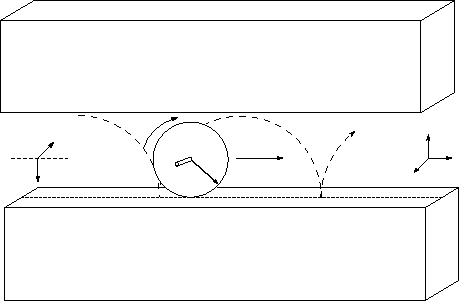
\includegraphics[width=\textwidth]{v3_3}
	\caption{Движение заряда в скрещенных полях}
	\figmark{Crossed fields}
\end{figure}
\todo[inline,author=Popov]{Рисунок странный. Что там по центру? Надо бы нарисовать другой}

Для уяснения идеи метода магнетрона, рассмотрим вначале движение заряда в
<<плоском магнетроне>>, который можно
представить себе в виде плоского конденсатора, помещённого в магнитное поле так,
что $\vec{E}\bot\vec{B}$ (рис.~\figref{Crossed fields}). При этом отрицательная
пластина конденсатора играет роль катода, положительная соответственно анода.
Если бы магнитного поля не было, то все электроны, вылетевшие без начальной
скорости из катода такого плоского диода, попадали бы на анод. При наличии
магнитного поля траектории электронов искривляются, вследствие чего при
достаточно большом магнитном поле ни один электрон не достигнет анода. Для
заданного напряжения между катодом и анодом существует некоторое критическое
значение магнитной индукции~$B_\text{кр}$, при котором траектории касаются
поверхности анода. Если~$B<B_\text{кр}$, то все электроны достигают анода и ток
через магнетрон имеет то же значение, что и без магнитного поля. Если же
$B>B_\text{кр}$, то электроны не достигают анода и ток через лампу равен нулю.

Рассчитаем это критическое значение индукции магнитного поля. Уравнения движения
электрона в нашем случае имеет вид
\begin{equation}
	\eqmark{3.9}
	m\frac{dv_x}{dt}=ev_y B,
\end{equation}
\begin{equation}
	\eqmark{3.10}
	m\frac{dv_y}{dt}=eE-ev_x B
\end{equation}
при начальных условиях $x(0)=y(0)=0$, $v_x(0)=v_y(0)=0$.

Непосредственной подстановкой несложно убедиться в том, что решением системы
дифференциальных уравнений с заданными
начальными условиями является уравнение циклоиды (в параметрической форме):
\begin{equation}
	\eqmark{3.11}
	x = vt - R\sin\omega t,\qquad y = R(1-\cos\omega t),
\end{equation}
где $ v=E/B$, $R=v/\omega=Em/(eB^2)$.

Касание анода происходит при $2R=d$ ($d$~--- расстояние между анодом и катодом).
Этому значению соответствует
критическое поле
\begin{equation}
	B_\text{кр}=\frac{\sqrt{2V}}{d\sqrt{e/m}}.
	\eqmark{3.12}
\end{equation}
Из последней формулы находим удельный заряд:
\begin{equation}
	\eqmark{3.13}
	\frac{e}{m}=\frac{2V}{d^2B_\text{кр}^2}.
\end{equation}
\todo[inline,author=Popov]{Убрать детали в описание работы. Во введении ---
    только общие соотношения}

Эта формула позволяет вычислить~$e/m$, если при заданном значении напряжения на
аноде~$V$ найти такое значение
магнитного поля, при превышении которого ток в магнетроне отсутствует.
\todo[inline,color=cyan]{<---}


\introsection{Электрический ток в вакуумном диоде}

\todo[inline,author=Popov]{Текст написан плохо и изыточно. Можно короче и лучше --->}
Электрический ток в вакуумном диоде представляет собой упорядоченное движение
электронов, испускаемых катодом. Явление испускания электронов поверхностью
твёрдого тела или жидкости называется \term{электронной эмиссией}.
Существует несколько видов электронной эмиссии. В~частности, в случае
испускания электронов поверхностями нагретых тел эмиссия называется
\term{термоэлектронной}.

Для удаления электрона из твёрдого вещества в вакуум необходимо совершить работу.
Работу по переводу электрона в свободное состояние с нулевой кинетической
энергией называют \term{работой выхода}. В~случае термоэлектронной эмиссии
работа выхода совершается за счёт кинетической энергии электронов,
которой они обладают внутри тела. Также работа может быть совершена внешним полем.
У~чистых металлов работа выхода составляет несколько электрон-вольт.

При повышении температуры металла увеличивается энергия теплового движения
электронов, количество быстрых электронов и заметное их количество сможет
преодолеть задерживающее электрическое поле и выйти из металла. Если приложить
электрическое поле, направленное к поверхности металла, то оно будет увлекать
вышедшие электроны и через вакуум потечёт электрический ток.
Этот ток называется \term{термоэлектронным}.

При \important{холодном} катоде ток через диод при подаче на анод
положительного потенциала практически отсутствует. Если же \important{нагреть}
катод, то в диоде возникает заметный ток. Ток прекращается при изменении
полярности батареи. Это как раз и указывает на то, что носителями тока в диоде
являются отрицательно заряженные частицы --- электроны.

Если бы все электроны, вылетающие из поверхности катода, попадали на анод, то
сила термоэлектронного тока~$I$ не зависела бы от величины приложенного
напряжения~$V$. На самом деле это не так. С~возрастанием напряжения ток растёт.
Однако возрастание идёт не пропорционально~$V$, так что закон Ома для вакуумного
диода не выполняется. Нелинейная зависимость тока от напряжения объясняется тем, что в пространстве
между катодом и анодом образуется отрицательный пространственный заряд,
изменяющий распределение потенциала в диоде.

При достижении определённого напряжения дальнейшее
нарастание тока практически прекращается. Ток достигает предельного значения,
называемого \term{током насыщения}. Величина тока насыщения определяется количеством
электронов, которое способно выйти из поверхности катода в единицу времени, и,
следовательно, увеличивается с ростом температуры. Если электрическое поле настолько
сильное, что способно отвести все эмитированные электроны, то дальнейшее
увеличение напряжения уже не приводит к увеличению термоэлектронного тока.
\todo[inline]{<--}

\todo[inline,color=green,author=Popov]{Вставить вместо текста выше -->}
Электрический ток в вакуумном диоде представляет собой упорядоченное движение
свободных электронов, испускаемых катодом.  При этом в откачанном сосуде
электроны практически не испытывают сопротивления своему движению,
в отличие от обычного проводника. Характерной особенностью такой системы
является наличие пространственного заряда. Как следствие, для вакуумного
диода не применим закон Ома.

Явление испускания электронов поверхностью твёрдого тела или жидкости называется
\term{электронной эмиссией}. Для удаления электрона из твёрдого вещества в
вакуум необходимо совершить работу, называемую \term{работой выхода} $A_{вых}$
(у чистых металлов $A_{вых}\sim 1\;эВ$).
Один из механизмов эмиссии --- испускание электронов с поверхности сильно
нагретых тел (\term{термоэлектронная эмиссия}).
Работа выхода при этом совершается за счёт кинетической энергии электронов,
которой они обладают внутри тела.

Если создать электрическое поле вне металла, оно будет увлекать вышедшие
электроны и через вакуум потечёт электрический ток.
С повышением температуры поверхности экспоненциально быстро растёт доля частиц,
способных преодолеть потенциальный барьер $A_{вых}$,
и следовательно, растёт интенсивность эмиссии электронов. Это приводит к тому, что
в пространстве диода~--- особенно вблизи катода~--- накапливается отрицательный
объёмный заряд, экранирующий внешнее поле. Из-за этого результирующий ток
в диоде оказывается значительно меньше тока эмиссии с катода.
Такой режим работы диода называют \term{режимом объёмного заряда}.

При достижении определённого напряжения дальнейшее нарастание тока практически
прекращается~--- ток достигает предельного значения $I_{нас}$, называемого
\term{током насыщения}. Это обусловлено ограниченностью эмиссионной способности
катода~--- величина тока насыщения определяется количеством электронов,
которое способно выйти из поверхности катода в единицу времени.
\todo[inline,color=green]{<---}


\paragraph{<<Закон 3/2>> для вакуумного диода.}
Рассмотрим режим объёмного заряда в простейшем случае \important{плоского} диода.
Его электроды представимы в виде двух параллельных плоскостей,
между которыми задано напряжение $V$. Расстояние~$d$ между электродами много
меньше их площади. Направим ось~$x$ перпендикулярно к поверхности катода
в сторону анода, совместив начало координат с поверхностью
катода. В~этой модели задача стала одномерной~--- все величины являются
функциями только координаты~$x$.

Запишем для электрического поля теорему Гаусса в дифференциальной форме:
\[
\frac{dE}{dx} = \frac{\rho}{\varepsilon_0},
\]
где~$\rho(x)$~--- плотность электрического заряда. По определению потенциала
электростатического поля имеем
\[
E = -\frac{d\varphi}{dx}.
\]
Отсюда находим, что $\varphi(x)$ удовлетворяет уравнению
\begin{equation}
	\eqmark{3.14}
	\frac{d^2\varphi}{dx^2}=-\frac{\rho}{\varepsilon_0}.
\end{equation}
Это частный (одномерный) случай \term{уравнения Пуассона}.

Плотность тока в диоде равна $j=\rho v$, где $v$~--- скорость электронов.
В стационаре заряд нигде не накапливается, поэтому плотность тока всюду одинакова: $j=\const$.
Из закона сохранения энергии имеем:
\begin{equation*}
	\frac{mv^2}{2}=e\varphi.
\end{equation*}
Здесь мы выбрали начало отсчёта потенциала на катоде, а также
пренебрегли \important{начальными тепловыми скоростями},
с которыми вылетают электроны с поверхности катода. Это можно сделать, если
приложенное напряжение достаточно велико: $eV\gg mv_0^2/2$.

Исключив из полученных соотношений плотность электронов~$\rho$ и скорость~$v$,
приходим к уравнению
\begin{equation}
	\eqmark{3.15}
    \frac{d^2\varphi}{dx^2}=\sqrt{\frac{m}{2e\varphi}} \frac{j}{\varepsilon_0}
\end{equation}
с граничными условиями
\begin{equation*}
 \varphi(0)=0,\qquad \varphi(d)=V.
\end{equation*}

Для однозначного решения этого дифференциального уравнения второго порядка
необходимо ещё одно граничное условие.
\todo[inline,author=Popov]{Это неправильное объяснение выбора граничного
    условия! В общем случае решения с конечными $E$ и $j$
на катоде существуют! На самом деле здесь физическое условие бесконечной
эмиссионной способности катода
--->}
 Если сопоставить уравнения \eqref{3.14} и \eqref{3.15}, то можно сделать вывод
об обращении плотности заряда на катоде в бесконечность. Точка~$x=0$ является
особой точкой уравнения \eqref{3.15}, в которой оно теряет смысл. Это связано с
тем, что мы пренебрегли тепловыми скоростями на катоде, приняв их равными нулю.
Оказывается, что в этой модели плотность тока через диод получается конечной,
только если напряжённость поля у катода равна нулю.
Это условие означает, что поле возникающего вблизи катода пространственного заряда полностью экранирует
электрическое поле, создаваемое разностью потенциалов между анодом и катодом.
Таким образом, получаем второе граничное условие в виде
\begin{equation*}
    \left.\frac{d\varphi}{dx}\right|_{x = 0}=0.
\end{equation*}
\todo[inline]{<---}

\todo[inline,author=Popov,color=green]{Вставить этот текст --->}
В общем случае это должна быть связь между плотностью тока~$j$ и электрическим
полем на поверхности катода $E_0 = -\left.\frac{d\varphi}{dx}\right|_{x=0}$,
которую однако  теоретически установить затруднительно.
Учтём, что в режиме объёмного заряда количество электронов, способных покинуть
катод из-за его нагрева, значительно превосходит ток в диоде.
Следовательно, \important{эмиссионная способность катода практически не ограничена},
поэтому чтобы плотность тока оставалась конечной,
напряжённость электрического поля внутри катода нужно устремить к нулю: $E_0\to 0$.
Таким образом, получаем второе граничное условие в виде
\begin{equation*}
    \left.\frac{d\varphi}{dx}\right|_{x = 0}=0.
\end{equation*}

Прямой подстановкой можно проверить, что решением \eqref{3.15},
удовлетворяющим данным граничным условиям, является функция вида
\begin{equation*}
    \varphi^{3/2} =\const \cdot j x^2.
\end{equation*}
Подставляя $\varphi(d)=V$, получим связь между током и напряжением
(вольт-амперную характеристику) в вакуумном диоде:
\begin{equation}
    I \propto V^{3/2}.
\end{equation}
Это так называемый <<\term{закон 3/2}>> \term{Чайлда--Ленгмюра}.

Как следует непосредственно из проведённого вывода,
в реальной системе <<закон 3/2>> нарушается как при слишком малых напряжениях,
когда нельзя пренебрегать начальными тепловыми скоростями электронов,
так и при слишком больших напряжениях, когда диод переходит в режим насыщения.
В~промежуточной области закон хорошо подтверждается на опыте, в том числе
и для электродов неплоской геометрии.
\todo[inline,color=green]{<---}

\todo[inline,author=Popov,color=cyan]{Убрать в описание работы и там дополнить --->}
Теперь задача о распределении потенциала становится однозначной и приводит к
решению
\begin{equation*}
	j=\frac{4\varepsilon_0}{9x^2}\sqrt{\frac{2e}{m}}\varphi^{3/2}.
\end{equation*}
\todo[inline,author=Popov]{Убрать детали в описание работы,
во введении --- только общие законы}

Так как $\varphi(d)=V$, где~$d$~--- расстояние между электродами, то для
зависимости тока от напряжения получаем
\begin{equation*}
	I=\frac{4\varepsilon_0 S}{9d^2}\sqrt{\frac{2e}{m}}V^{3/2},
\end{equation*}
где~$S$~--- площадь катода. Мы получили зависимость тока через плоский диод от
приложенного к нему напряжения, известную как <<закон трёх вторых>> для плоского
диода. Оказывается, что не только для плоского вакуумного диода, а и для
вакуумного диода с электродами любой другой геометрии ток подчиняется <<закону
степени трёх вторых>>.

Полученная формула подсказывает процедуру измерения удельного заряда электрона.
Для этого достаточно по
результатам эксперимента построить график зависимости тока от напряжения в
степени трёх вторых, который должен
представлять собой прямую линию, проходящую через начало координат. Угол наклона
этой прямой линии пропорционален (с известным коэффициентом) квадратному корню
из~$e/m$~--- искомой величины удельного заряда электрона.
\todo[inline,color=cyan]{<---}

\introsection{Свободные носители заряда в металлах и~полупроводниках}

Проводимость большинства твёрдых тел связана с движением электронов. Электроны
входят в состав атомов всех тел, однако одни тела не проводят электрический ток
(диэлектрики), а другие являются хорошими его проводниками. Причина различия
заключается в особенностях энергетического состояния внешних электронов атомов в
этих веществах.

\paragraph{Зонная модель.}
При объединении атомов в твёрдое тело (кристалл) внешние электроны теряют связь
со <<своими>> атомами и теперь принадлежат \important{всему} кристаллу.
Каждому уровню энергии электрона \important{одиночного} атома в кристалле
соответствует \important{группа} близких уровней в кристалле,
<<сливающихся>> в непрерывную \term{зону}.
Число доступных состояний в зоне при <<слиянии>> остаётся неизменным --- оно
равно числу мест на соответствующем атомном уровне,
умноженному на число атомов в кристалле. Оно определяет максимальное число
электронов, которое может <<поместиться>> в зоне в силу принципа
\important{запрета Паули}.

\todo[inline,author=Popov]{Нужен поясняющий рисунок для зонной модели}
Если одна из зон до конца заполнена электронами, а следующая~---
пуста, то под действием слабого внешнего электрического поля
электроны не могут изменить своё состояние, а значит и не могут
прийти в движение. Тогда вещество является \term{диэлектриком}.
Верхняя из заполненных зон называется \term{валентной зоной}.

Положение меняется, если в кристалле имеется зона, \important{частично} заполненная
электронами. В~этом случае внешнее электрическое поле может изменить
распределение электронов по уровням энергии и вызвать их упорядоченное движение.
Частично заполненная зона называется \term{зоной проводимости}.
Такая зона имеется у всех твёрдых проводников электрического тока;
в том числе её имеют все металлы.

Если ширина запрещённой зоны относительно невелика, тепловое движение
перебрасывает часть электронов из валентной зоны в свободную зону над ней~---
зону проводимости. При этом в зоне проводимости появляются электроны,
а в валентной зоне~--- свободные места~--- \term{дырки}.
Электроны в зоне проводимости и дырки валентной зоны участвуют в переносе заряда.
Такие вещества называются \term{полупроводниками}.
% Обычно к полупроводникам
% относят материалы с шириной запрещённой зоны $\Delta E \lesssim 2$~эВ.
% Число носителей тока в
% полупроводниках экспоненциально увеличивается с~повышением температуры.

\todo[inline,author=Popov]{Очень невнятный кусок --->}
Рассматривая коллективное движение электронов почти заполненной зоны,
полезно мысленно заполнить свободные места
воображаемыми парами, состоящими из электронов с одинаковыми по величине
положительным и отрицательным зарядами. Обычные отрицательные заряженные
электроны заполняют теперь все уровни и, следовательно, не могут принимать
участия в проводимости. Они образуют структуру, характерную для изоляторов.
Проводимость связана только с введёнными нами
<<электронами>>, обладающими положительным зарядом. Такие <<электроны>> носят
название \important{дырок}. При рассмотрении явлений, происходящих в~металлах
с~почти заполненной валентной зоной, удобно представлять себе дело так, как если
бы проводниками тока были не настоящие электроны, а положительно заряженные
дырки. В~этом случае говорят о \important{дырочном типе проводимости.}

Электронным типом проводимости обладает большинство чистых металлов. Однако в
ряде металлов (бериллий, кадмий и некоторые другие) основными носителями
электрического тока являются дырки. Это связано с особенностями их зонной
структуры.
\todo[inline]{<---}

\todo[inline,author=Popov,color=green]{Здесь нужно вставить что-то внятное
о наглядном образе дырок}

\introsubsection{Эффект Холла}

Рассмотрим прохождение тока в твёрдом проводнике в рамках модели
свободных электронов при наличии магнитного поля.

\todo[inline,author=Popov]{Написано во-первых, заумно, во-вторых, небрежно.
    Нужна переработка при сохранении сути --->}
Закон Ома в дифференциальной форме выражает связь векторов~$\vec{j}$~---
плотности тока и~$\vec{E}$~--- электрического поля:
\begin{equation}
    \vec{j}=\lambda \vec{E}.
	\eqmark{3.16}
\end{equation}
В отсутствие магнитного поле, если проводящая среда \important{изотропна}
(то есть не имеет выделенных направлений), проводимость~$\lambda$ является
\important{скалярной} величиной. Это значит, что векторы~$j$ и~$E$ сонаправлены.
В~общем же случае под $\lambda$ нужно понимать \important{тензор} $\widehat{\lambda}$~--- то есть
матрицу~$3\times 3$, при умножении которой на вектор~$E$ получается вектор~$j$:
\begin{equation*}
    j_{i} = \sum_{k=1}^3 \lambda_{ik} E_k,\qquad i=1,\,2,\,3.
\end{equation*}
\todo[inline,author=Popov]{Сначала надо на пальцах объяснить эффект, а потом говорить
    о недиагональных матрицах}
В ненулевом магнитном поле эта матрица становится недиагональной в результате
эффекта Холла.

Электроны в металлах и легированных полупроводниках движутся с большими
скоростями во всех направлениях, а под действием тянущего
электрического поля приобретают ненулевую среднюю скорость дрейфового движения
$v_{dr}=  Eb$, где~$b$~--- подвижность.

\todo[inline,author=Popov]{Какое еще магнИтосопротивление? Где определение?}
Разберем магнитосопротивление и эффект Холла на микроуровне. Если магнитное поле
направлено вдоль тока, то
оно не влияет на ток, поскольку сила Лоренца равна нулю. Поэтому мы рассмотрим
случай, когда поле перпендикулярно
току. Пусть рассматриваемая система для простоты содержит носители только одного
сорта (большинство металлов являются хорошими примерами).
\begin{figure}[h!]
	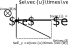
\includegraphics[width=0.9\textwidth]{Chapter_3/Hall_forces}
	\caption{Силы, действующие на носитель заряда в проводящей среде в тянущем
электрическом и перпендикулярном ему магнитном полях.}
	\figmark{Hall forces}
\end{figure}

Если в системе локально течет ток электронов $j_x=nev_{dr\, x}$, направленный
вдоль оси~$x$, а магнитное поле~$B$ направлено вдоль оси~$z$, то на заряды
действует действует сила Лоренца $ F_{L}=e[v_{dr}B]$ вдоль оси~$y$.
Сила Лоренца должна приводить к образованию компоненты тока вдоль оси~$y$, но по
условиям ток течет вдоль~$x$. Это значит, что заряды должны перераспределиться
таким образом, чтобы полностью скомпенсировать силу
Лоренца, создав в~$y$ направлении электрическое холловское поле $E_y=v_{dr}B$.
Поскольку сила Лоренца
оказывается полностью скомпенсирована $eE_y$, то электрон движется так, как если
бы магнитного поля не
было, то есть $j_x=E_xbne$, $j_y=j_z=0$. Это позволяет написать в явном виде
тензор удельного сопротивления.
Тензор удельного сопротивления~$\widehat{\rho}$ является обратным к тензору
проводимости: $E=\widehat{\rho}j$, то есть
$\widehat{\rho}=\widehat{\lambda}^{-1}$.
\begin{equation}
	\widehat{\rho}(B)=\frac{1}{bne}\left(
	\begin{matrix}
		{1} & {bB} & {0} \\
		{-bB} &{1}& {0} \\
		{0} &{0}& {1}
	\end{matrix}
	\right).
	\eqmark{3.17}
\end{equation}

Здесь коэффициент, стоящий перед матрицей,
\begin{equation}
	\frac{1}{bne} = \rho_0
	\eqmark{UdSoprot}
\end{equation}
есть удельное сопротивление полупроводника при отсутствии магнитного поля.

Обращением этой матрицы нетрудно получить тензор проводимости:
\begin{equation}
	\widehat{\lambda}(B)=\frac{bne}{1+b^2B^2}\left(
	\begin{matrix}
		{1} & {bB} & {0} \\
		{-bB} &{1}& {0} \\
		{0} &{0}& {1}\\
	\end{matrix}
	\right).
	\eqmark{3.18}
\end{equation}

\todo[inline]{<---}

\paragraph{Измерения эффекта Холла.}
Существуют две основных и принципиально различных геометрии для исследования
магнитосопротивления: геометрия
мостика Холла и геометрия диска Корбино (см. рис.~\figref{Geometries}).

\todo[inline,author=Popov]{И здесь не акууратно! Обозначения не введены ($w$?),
термины не определены (холловское напряжение?)}
В~геометрии мостика Холла ток вынуждают течь вдоль образца, сила Лоренца
прибивает носители к краю образца, создавая тем самым холловское поле, которое
компенсирует силу Лоренца. Напряжение между точками $V_{xy}$ равно~$E_yw$, где,
согласно уравнению \eqref{3.17}, $E_y=\rho_{yx}j_x=j_x B/(ne)$. Плотность
тока, текущего через образец, равна полному току~$I$, деленному на площадь
поперечного сечения образца~$wh$. Таким образом, для холловского напряжения
имеем:
\begin{equation}
	V_{xy}=\frac{IB}{neh}.
	\eqmark{3.19}
\end{equation}

В~этой же модели для падения напряжения вдоль образца имеем:
\begin{equation}
	V_{xx}=\frac{Il}{nebwh}.
	\eqmark{3.20}
\end{equation}

\todo[inline,author=Popov]{Интересно, что при наличии эффекта Холла
    есть зависимость тензора проводимости от $B$,
    а магнетосопротивление вроде как равно нулю! Требуется четкое
    определение того, \emph{что такое магнетосопротивление}}
Tаким образом, удельное сопротивление~$\rho_{xx}$ образца не зависит от
магнитного поля (магнитосопротивление равно 0). Этот факт объясняется тем, что
сила Лоренца и сила ЭДС Холла (рис. \figref{Hall forces}) полностью
уравновешивают друг друга. В~реальных системах, тем не менее, предположения
модели не выполняются и магнитосопротивление зачастую отлично от 0. Причины
могут быть различными:
\begin{enumerate}
\item Система может быть анизотропной, то есть в разных направлениях ($x,y,z$)
токопроводящие свойства различны. В~этом случае величина силы Лоренца содержит
не среднюю дрейфовую скорость, а зависит от направления большой мгновенной
скорости электрона.

\item Система может быть многокомпонентной. Например, в полупроводниках часто
одновременно существуют электроны и дырки, концентрации ($n$ и~$p$) и
подвижности ($b_n$ и~$b_p$) которых в общем случае различаются. Тогда полный
тензор проводимости будет суммой тензоров проводимости двух компонент вида
\eqref{3.18}. Обращением тензора проводимости в пределе малых магнитных полей
можно показать, что холловское сопротивление двухкомпонентной системы в
полупроводнике равно:
\begin{equation}
	R_{xy}\equiv \frac{V_{xy}}{I}=\frac{nb_n^2-pb_p^2}{eh(nb_n+pb_p)^2}B
	\eqmark{3.21}
\end{equation}
\todo[inline,author=Popov]{Откуда формула? Зачем она нужна? Лучше убрать
    или вынести в приложение, где дать её вывод.}

\item Существуют квантовые эффекты в проводимости, которые приводят к тому, что
подвижность зависит от магнитного поля. Например если сам проводящий материал
является ферромагнетиком, то с ростом поля он намагничивается, количество
доменов уменьшается, а доменные стенки являются причиной сильного рассеяния, то
есть уменьшают подвижность.
\end{enumerate}

Поскольку холловское сопротивление содержит толщину образца~$h$, то договорились
называть холловское сопротивление, умноженное на толщину образца, постоянной
Холла. Постоянная Холла характеризует материал, так как зависит только от
концентрации носителей в нем:
\begin{equation}
	R_x=\frac{1}{ne}
	\eqmark{HallConstant}
\end{equation}
или от соотношений между концентрациями и подвижностями, если в материале
несколько типов носителей. В~таблице в приложении даны постоянные Холла для
различных металлов. Для полупроводников постоянные Холла сильно зависят от
наличия малых концентраций примеси и температуры.

Отдельно следует упомянуть, что существуют двумерные системы (например, графен),
в которых движение носителей заряда происходит только в плоскости, а движение в
перпендикулярном направлении квантовомеханически запрещено. В~этих системах
концентрация измеряется в количестве носителей на единицу площади, а холловская
постоянная есть просто холловское сопротивление, делённое на магнитное поле. В
двумерных системах тензоры в формулах \eqref{3.17} и \eqref{3.18} содержат
только~$x$ и~$y$ компоненты, то есть являются матрицами~$2\times2$.
\todo[inline, author=Popov]{А стоило ли отдельно упоминать графен,
    прерывая повествование? Лирические
    отступления вынести в конец или в начало раздела}

Измерения в геометрии мостика Холла представляют собой четырехконтактные
измерения, то есть два контакта используются для задания тока через образец, а с
двух контактов снимается падение напряжения. Поскольку вольтметр обладает
бесконечным сопротивлением (то есть ток через него не течет), измеряемое падение
напряжения совершенно не зависит от свойств контактов, а определяется только
свойствами материала.

Геометрия диска Корбино представляет собой двухточечную схему, то есть
сопротивление образца в ней суммируется с сопротивлениями контактов. Поэтому
исключительно важно создать низкоомные контакты к образцу, сопротивлением
которых можно пренебречь. В~геометрии Корбино из-за аксиальной симметрии не
формируется холловское напряжение. Электрическое поле направлено строго по
радиусу системы. В~магнитном поле ток вынужден протекать под углом к
электрическому полю, то есть по спирали. Из-за симметрии полный ток включает
только компоненту вдоль радиуса $j_r=\lambda_{xx} E_r$. Плотность тока может
быть выражена через полный ток и толщину образца $j_r=I/(2\pi rh)$.
Теперь запишем для напряжения:
\begin{equation*}
V={\int_{r_1}}^{r_2}E_r dr={\int_{r_1}}^{r_2}\frac{j_r}{\lambda_{xx}}
dr={\int_{r_1}}^{r_2}I\rho_0\frac{1+b^2B^2}{2\pi
rh}dr=I\rho_0\frac{1+b^2B^2}{2\pi h}\ln{\frac{r_2}{r_1}}.
\end{equation*}
\todo[inline,author=Popov]{Убрать этот ужас в описание работы}

Если система однокомпонентная, то магнетосопротивление в геометрии Корбино есть
\begin{equation}
	R(B) = R_0(1+b^2B^2)
	\eqmark{MagnetoSoprot}.
\end{equation}

Здесь
\begin{equation}
	R_0 = \frac{\rho_0}{2\pi h} \ln{\frac{r_2}{r_1}}
	\eqmark{KorbinoSoprot}
\end{equation}

Для наблюдения этого магнитосопротивления выбирают систему с большой подвижнотью
носителей (как правило, это полупроводник с низкой эффективной массой электронов
типа InSb).

\begin{figure}[h!]
	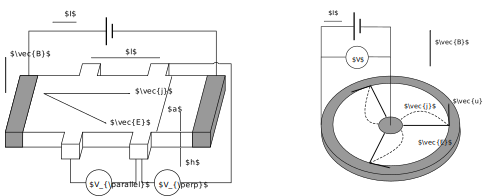
\includegraphics[width=0.9\linewidth]{Chapter_3/2schemes}
	\caption{Две геометрии для исследования влияния магнитного поля на
проводящие свойства: мостик Холла (слева) и диск Корбино (справа).}
	\figmark{Geometries}
\end{figure}

\todo[inline,author=Popov]{Что это? Куски старого текста? Раздел остро
    нуждается в редактировании! --->}

При наложении внешнего электрического поля~$E$ электроны начинают ускоряться.
Однако после некоторого <<свободного пробега>> происходит соударение с решёткой,
электрон теряет набранную энергию, и процесс ускорения начинается заново.
Соударения с решёткой, подобно вязкому трению, приводят к тому, что
результирующее движение электрона можно описать некоторой средней скоростью
$\left< v \right>$, пропорциональной внешнему полю:
\begin{equation}
	\eqmark{3.22}
	\left< \vec{v} \right>=-b\vec{E}.
\end{equation}



Введённая здесь величина~$b$ называется \important{подвижностью}. В~определённых
пределах изменения температуры,
напряжённости поля и его частоты эта характеристика вещества остаётся постоянной
и приводится в справочниках. Для
положительно заряженных носителей тока в формуле \eqref{3.22}, очевидно, стоит
знак <<плюс>>.

При установившемся движении средняя сила, действующая на электроны со стороны
кристаллической решётки, равна внешней силе~$-eE$ и направлена в противоположную
сторону. Поэтому действие кристаллической решётки на движение электронов в
среднем эквивалентно силе трения, пропорциональной скорости:
\begin{equation}
	\eqmark{3.23}
	F_\text{тр}=-\frac{e}{b}\average{\vec{v}}.
\end{equation}

Если концентрация электронов равна~$n$, величина плотности тока определится
очевидным соотношением
\begin{equation}
	\eqmark{3.24}
	j=en\average{v}=enbE.
\end{equation}

Таким образом, выполняется закон Ома~--- величина плотности тока~$j$
пропорциональна напряжённости поля~$E$:
\begin{equation}
	\eqmark{3.25}
	j=\lambda E.
\end{equation}

Сравнивая \eqref{3.24} и \eqref{3.25}, получаем выражение для проводимости
\begin{equation}
	\eqmark{3.26}
	\lambda=enb.
\end{equation}

Химически чистые полупроводники обладают проводимостью, которая связана с
небольшим числом электронов в зоне
проводимости и таким же числом дырок в валентной зоне. Такая проводимость
называется собственной~--- она не связана с примесями. Добавление небольшого
количества специально подобранных примесей (так называемое
легирование) может существенно увеличить проводимость полупроводников или даже
создать ощутимую проводимость при комнатной температуре в веществах с
запрещённой зоной, ширина которой заметно превышает 2~эВ. Такое происходит,
когда атомы примеси имеют энергетические уровни в запрещённой зоне основного
материала.

Если заполненные примесные уровни расположены вблизи потолка запрещённой зоны,
находящиеся на этих уровнях электроны легко переходят в зону проводимости.
Наоборот, на свободные уровни у дна зоны проводимости легко переходят электроны
валентной зоны с образованием в этой зоне дополнительного количества дырок. В
обоих случаях число переносчиков заряда увеличивается, и проводимость
возрастает. В~первом случае говорят о полупроводниках \important{электронного},
или $n$-типа, а во втором~--- о  полупроводниках дырочного, или $p$-типа. В
общем случае в процессе электрической проводимости участвуют как электроны, так
и дырки. Удельная электрическая проводимость полупроводника при этом равна
\begin{equation}
	\eqmark{3.27}
	\lambda=e(nb_e+pb_p),
\end{equation}
где~$n$ и~$p$~--- концентрации электронов и дырок, а~$b_e$ и~$b_p$~--- их
подвижности. В~случае \important{примесной
проводимости} один тип носителей обычно существенно преобладает над другим и в
формуле \eqref{3.27} можно пренебречь одним из слагаемых.

\todo[inline]{<---}

\begin{lab:literature}
	\item{ \textit{Сивухин Д.В.} Общий курс физики.~--- T.~III. Электричество.~---
М.: Наука, 1983. \S\S~86, 95, 98, 100.}
	\item{ \textit{Кингсеп А.С., Локшин Г.Р., Ольхов О.А.} Основы физики.
Т.~1.~--- М.: Физматлит, 2001. \S\S~8.1--8.3.}
\end{lab:literature}


